\documentclass[12pt,a4paper]{article}
\usepackage[utf8]{inputenc}
\usepackage[spanish]{babel}
\usepackage{amsmath}
\usepackage{amsfonts}
\usepackage{amssymb}
\usepackage{makeidx}
\usepackage{graphicx}
\usepackage[left=2cm,right=2cm,top=2cm,bottom=2cm]{geometry}

\author{Felipe Alvarado Galicia}
\title{OPERADOR JACOBIANO}
\date{Profesor:Carlos Enrique Moran Garabito\\
Materia: Cinematica de Robots\\
15 de octubre de 2019}

\begin{document}
\maketitle
 
\includegraphics[scale=1]{logo1.png}\\
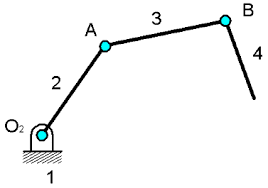
\includegraphics[scale=1]{imag5.png} 
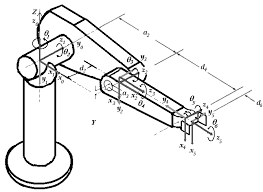
\includegraphics[scale=1]{imag8.png}\\\\\\\\\\\\\\\\\\\\\\\\\\\\\\\\\\\\\\\\\\\\\\

\tableofcontents

\section{El Jacobiano de una función}
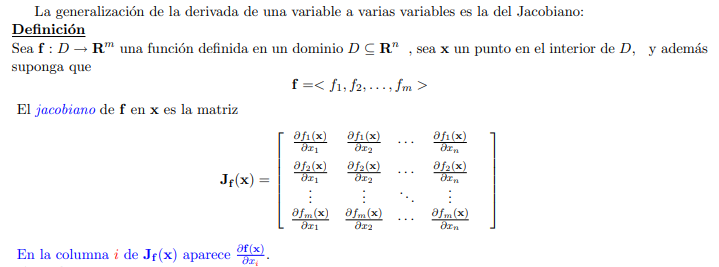
\includegraphics[scale=1]{jac fun.PNG} \\
EL JACOBIANO\\
En calculo vectorial, se llama jacobiano o determinante jacobiano al determinante de la matriz jacobiana. Tanto la matriz jacobiana como el determinante jacobiano reciben su nombre en honor al matemático Carl Gustav Jacobi.\\
La matriz jacobiana es una matriz formada por las derivadas parciales de primer orden de una función. Una de las aplicaciones más interesantes de esta matriz es la posibilidad de aproximar linealmente a la función en un punto. En este sentido, el jacobiano representa la derivada de una función multivariable.\\\\
\section{Matriz jacobiana}
La matriz jacobiana es una matriz formada por las derivadas parciales de primer orden de una función. Una de las aplicaciones más interesantes de esta matriz es la posibilidad de aproximar linealmente a la función en un punto. En este sentido, el jacobiano representa la derivada de una función multivariable.\\
Propiamente deberíamos hablar más que de matriz jacobiana, de diferencial jacobiana o aplicación lineal jacobiana ya que la forma de la matriz dependerá de la base o coordenadas elegidas. Es decir, dadas dos bases diferentes la aplicación lineal jacobiana tendrá componentes diferentes aun tratándose del mismo objeto matemático. La propiedad básica de la "matriz" jacobiana es la siguiente, dada una aplicación cualquiera F:Rn  tiende a Rm continua, es decir 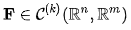
\includegraphics[scale=1]{1.PNG} 
se dirá que es diferenciable si existe una aplicación lineal 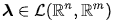
\includegraphics[scale=1]{2.PNG}  tal que:\\
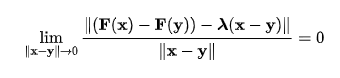
\includegraphics[scale=1]{Matriz Jacobiana.PNG} \\\\

\section{Bibliografía:}
http://www.mty.itesm.mx \\
http://calculovector.blogspot.com \\


\end{document}